\chapter{Materiais e Métodos}\label{cap:ferramentas}

Para obter melhor entendimento sobre ferramentas de visão computacional, em específico para detecção facial, este capítulo descreve a execução de testes feitos utilizando as ferramentas OpenCV e Keras, ambas aplicadas utilizando a linguagem de programação Python.
As ferramentas foram utilizadas para análise de um conjunto específico de imagens e os resultados foram validados utilizando as métricas já conhecidas para aprendizado de máquina e também uma metodologia de análise de custo baseada em métricas do mercado.

\section{OpenCV e Viola-Jones}

A ferramenta OpenCV, que pode ser encontrada no website Github \cite{itseez2015opencv}, é uma biblioteca de código aberto focada na solução de problemas utilizando visão computacional em tempo real, desenvolvida pela Intel e posteriormente pela Itseez, com suporte a múltiplas plataformas e uso gratuito sobre a licença de código aberto BSD. A ferramenta apresenta suporte a frameworks de aprendizado profundo, como TensorFlow, Pytorch e Caffe e contempla tanto funções básicas, para aplicações como processamento de imagem, alteração de cor ou resolução, até aplicações avançadas, como detecção facial, identificação de características e biometria \cite{wiki:OpenCV}.

Uma das ferramentas que será utilizada neste trabalho é a função de detecção de faces da ferramenta OpenCV, que utiliza um classificador em cascata baseado características. Esse é um método eficiente para reconhecimento de faces em imagens proposto por Paul Viola and Michael Jones, amplamente conhecido como método Viola-Jones, onde uma função é treinada com muitos exemplos positivos (imagens que contém o objeto a ser detectado) e negativos (imagens que não contém o objeto a ser detectado) e então utilizada para detectar as mesmas características em outras imagens \cite{itseez2014theopencv}.

A detecção de faces utilizando OpenCV consiste em duas etapas principais, a primeira consiste no treinamento do modelo, onde são apresentadas diversas imagens já identificadas para que o modelo encontre padrões positivos e negativos. Após o treinamento, a segunda etapa consiste em utilizar o modelo obtido para identificar, em novas imagens, características semelhantes as vistas nas imagens do treinamento. Neste projeto, será utilizado um modelo fornecido em conjunto com a ferramenta OpenCV, já treinado com diversos exemplos de faces frontais.

O algoritmo Viola-Jones foi publicado em 2001, no paper "Rapid object detection using a boosted cascade of simple features" ~\cite{paper-viola-jones} e é famoso por sua capacidade de detecção de faces com muita velocidade, isso ocorre devido a 3 principais técnicas utilizadas: o cálculo da imagem integral, o algoritmo \textit{AdaBoost} e o classificador em cascata.

\subsection{Imagem Integral} 

A primeira etapa do algoritmo Viola-Jones consiste em transformar a imagem original em uma imagem integral, isto é feito calculando o valor de cada ponto como a soma de todos os pontos que estão acima ou a esquerda do mesmo, como ilustrado na figura~\ref{fig:integral}.

\begin{figure}[htpb]
    \centering
    \caption{Imagem original (esquerda) e imagem integral (direita).}
    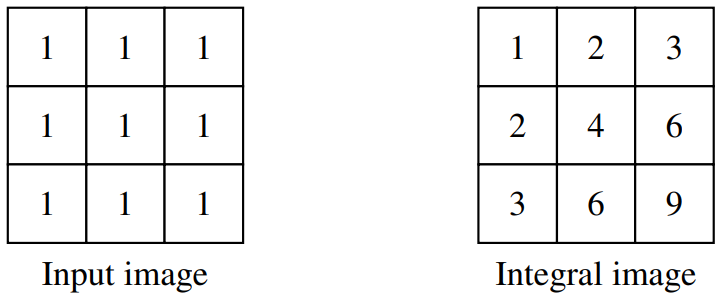
\includegraphics[scale=.3]{figs/imagem-integral.png}
    \label{fig:integral}
 \end{figure}

A utilização desta técnica permite calcular facilmente a soma dos valores internos de qualquer retângulo formado entre quatro pontos da imagem, utilizando apenas o valor dos seus cantos, possibilitando assim a análise rápida de diversas partes da imagem.

O calculo é feito definindo o retângulo a ser análisado e então aplicando a equação \ref{eq:img-integral}. Tal equação é utilizada em \ref{eq:img-integral-exemplo} para calcular soma dos valores do retângulo da figura \ref{fig:integral} que inclui os pontos 15, 16, 14, 28, 27 e 11.

\begin{align}\label{eq:img-integral}
    \text{ Soma dos valores retângulo } &= D - (B + C) + A \\
    \label{eq:img-integral-exemplo}
    15 + 16 + 14 + 28 + 27 + 11 &= 101 - (254 + 186) + 450 = 111
\end{align}

Com a possibilidade de calcular facilmente a soma dos pixels de um retângulo arbitrário de forma rápida, o algoritmo para detecção pode analisar diversos trechos da imagem, chamados aqui de características, fazendo a comparação de duas ou mais áreas retângulares predefinidas, como os exemplos ilustrado na figura \ref{fig:features}. 

\begin{figure}[htb]
    \centering
    \caption{Alguns exemplos de características retângulares analisadas.}
    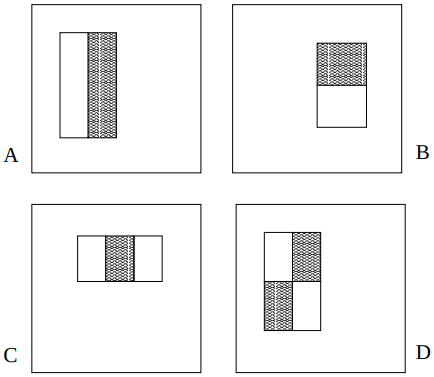
\includegraphics[scale=.5]{figs/features.png}
    \legend{Fonte: \citeauthoronline{paper-viola-jones} (\citeyear{paper-viola-jones})}
    \label{fig:features}
 \end{figure}

 O valor final de cada característica é definido pela soma do valor dos pixels sob o retângulo cinza menos a soma do valor dos pixels sob o retângulo branco.

%-
\subsection{Algoritmo de AdaBoost e Classificador em Cascata}
%-

As características demonstradas anteriormente, são definidas basicamente como duas ou mais áreas retângulares de qualquer tamanho, tal simplicidade implica na possibilidade da criação de uma enorme variação das mesmas que precisariam ser calculadas diversas vezes, para cada parte de imagem e com diferentes tamanhos, isso implica em um alto custo de processamento, para evitar tal problema é utilizado o algoritmo de \textit{AdaBoost} \cite{adaboost-Freund}, que possibilita grande otimização na demanda de processamento do detector facial e consequente redução do tempo de execução.

No caso do algoritmo de detecção facial Viola-Jones, o algoritmo AdaBoost é utilizado em dois momentos principais, o primeiro deles ocorre na seleção do conjunto de características mais eficientes durante o treino para criação do arranjo ponderado de vários classificadores fracos que combinados adequadamente se tornam um classificador forte \cite{fabio-luciana-2015}. A figura \ref{fig:top-features} retrata as melhores características registradas por \citeauthoronline{paper-viola-jones} (\citeyear{paper-viola-jones}), fica claro que as mesmas se destacam por evidenciar as regiões dos olhos e do nariz.

\begin{figure}[htb]
    \centering
    \caption{Características retângulares mais eficientes para detecção facial.}
    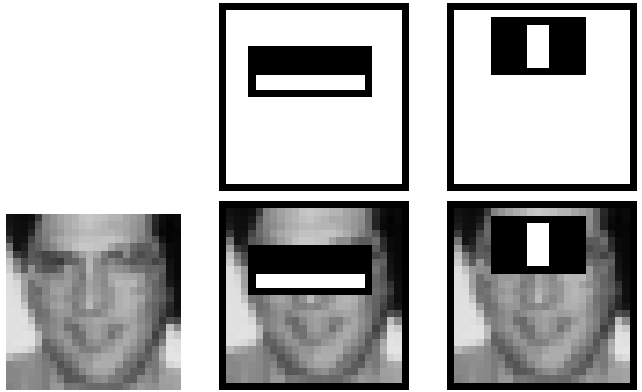
\includegraphics[scale=.4]{figs/top-features.png}
    \legend{Fonte: \citeauthoronline{paper-viola-jones} (\citeyear{paper-viola-jones})}
    \label{fig:top-features}
 \end{figure}

É importante salientar que geralmente uma face não ocupa a maior parte de uma imagem a ser identificada, portanto é necessário encontrar uma forma rápida de descartar os elementos do fundo da mesma e concentrar o poder de processamento nos elementos que tem maior probabilidade de serem reconhecidos como uma face, isso leva a uma formulação para o problema onde ao contrário de encontrar faces, é necessário um algoritmo que descarte as "não faces".  

Neste segundo momento, o AdaBoost apresenta uma ótima solução, esta consiste na utilização do arranjo de classificadores já ponderados anteriormente, aplicados de forma sequencial, iniciando do mais fraco para o mais forte, criando o que é chamado de classificador em cascata, conforme ilustrado na Figura \ref{fig:cascade-classifier}, permitindo que imagens que certamente não possuem faces sejam rapidamente descartadas logo nas primeiras iterações, enquanto imagens com possíveis faces são classificadas por toda cascata, trazendo um elevado nível de confiança ao resultado.

\begin{figure}[htb]
    \centering
    \caption{Diagrama do funcionamento do classificador em cascata.}
    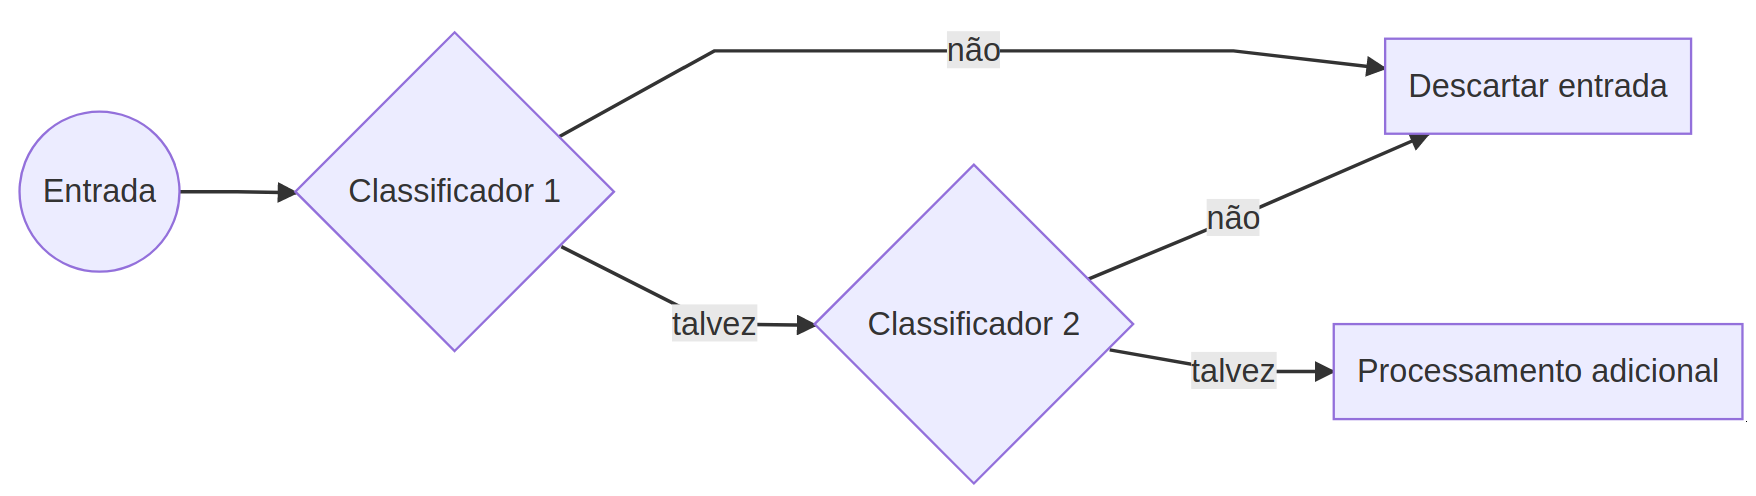
\includegraphics[scale=.2]{figs/cascade-classifier.png}
    \legend{Fonte: \citeauthoronline{paper-viola-jones} (\citeyear{paper-viola-jones})}
    \label{fig:cascade-classifier}
 \end{figure}

 Um classificador comum, com um único estágio normalmente aceitaria muitos casos de falso negativo, para reduzir a taxa de falsos positivos e de descarte de imagens relevantes, mas no classificador em cascata, falsos positivos nos primeiros estágios não são um problema, pois serão analisados em outros diversos estágios e provavelmente eliminados.

 A utilização desse modelo combinada com o algoritmo \textit{AdaBoost}, possibilita a análise das característica mais eficientes logo no início e consequentemente o descarte muito mais rápido dos casos negativos nos primeiros estágios.

 %-
 \subsection{Parametrização do Algoritmo}
 %-

 O procedimento de detecção facial utilizando o OpenCV permite ainda ajuste de parâmetros para a execução do algoritmo de Viola-Jones.

 O primeiro deles é chamado fator de escala que é o fator pelo qual as dimensões da imagem serão multiplicadas na tentativa de encontrar faces de diferentes tamanhos, pois o modelo é preparado para reconhecer faces de um tamanho específico, então durante a detecção a imagem é redimensionada e reanalisada diversas vezes para que faces de diferentes tamanhos possam ser detectadas. Para ajuste deste parâmetro, deve-se considerar que quanto mais próximo de 1 o seu valor, maior a chance de encontrar faces mas a execução do detector também se torna mais custosa em termos de processamento. 

 O segundo parâmetro é o número mínimo de vizinhos, que especifica quantos vizinhos cada retângulo candidato deve ter para retê-lo. Em mais detalhes, o detector analisa imagens utilizando um método de janelas retângulares que selecionam a partes da imagem, cada parte tem seus padrões comparados com os padrões de uma face e então é definido se esta janela contém ou não uma face, mas devido as várias iterações do detector sobre a mesma imagem durante a análise, uma mesma face pode ser detectada em mais de uma janela, tais janelas são consideradas janelas vizinhas, portanto para melhorar a precisão do detector e também filtrar detecções duplicadas, o parâmetro de número mínimo de vizinhos define quantas janelas vizinhas devem existir para considerar aquela parte da imagem como uma face. Enfim, para ajuste deste parâmetro, deve-se considerar que quanto mais próximo de zero o seu valor, maior a chance de detectar faces, mas consequentemente maior a chance de falsos positivos.

 \begin{figure}[htb]
    \centering
    \caption{Resultados da detecção utilizando o parâmetro de número mínimo de vizinhos igual a 0 (esquerda), 2 (centro) e 4 (direita).}
    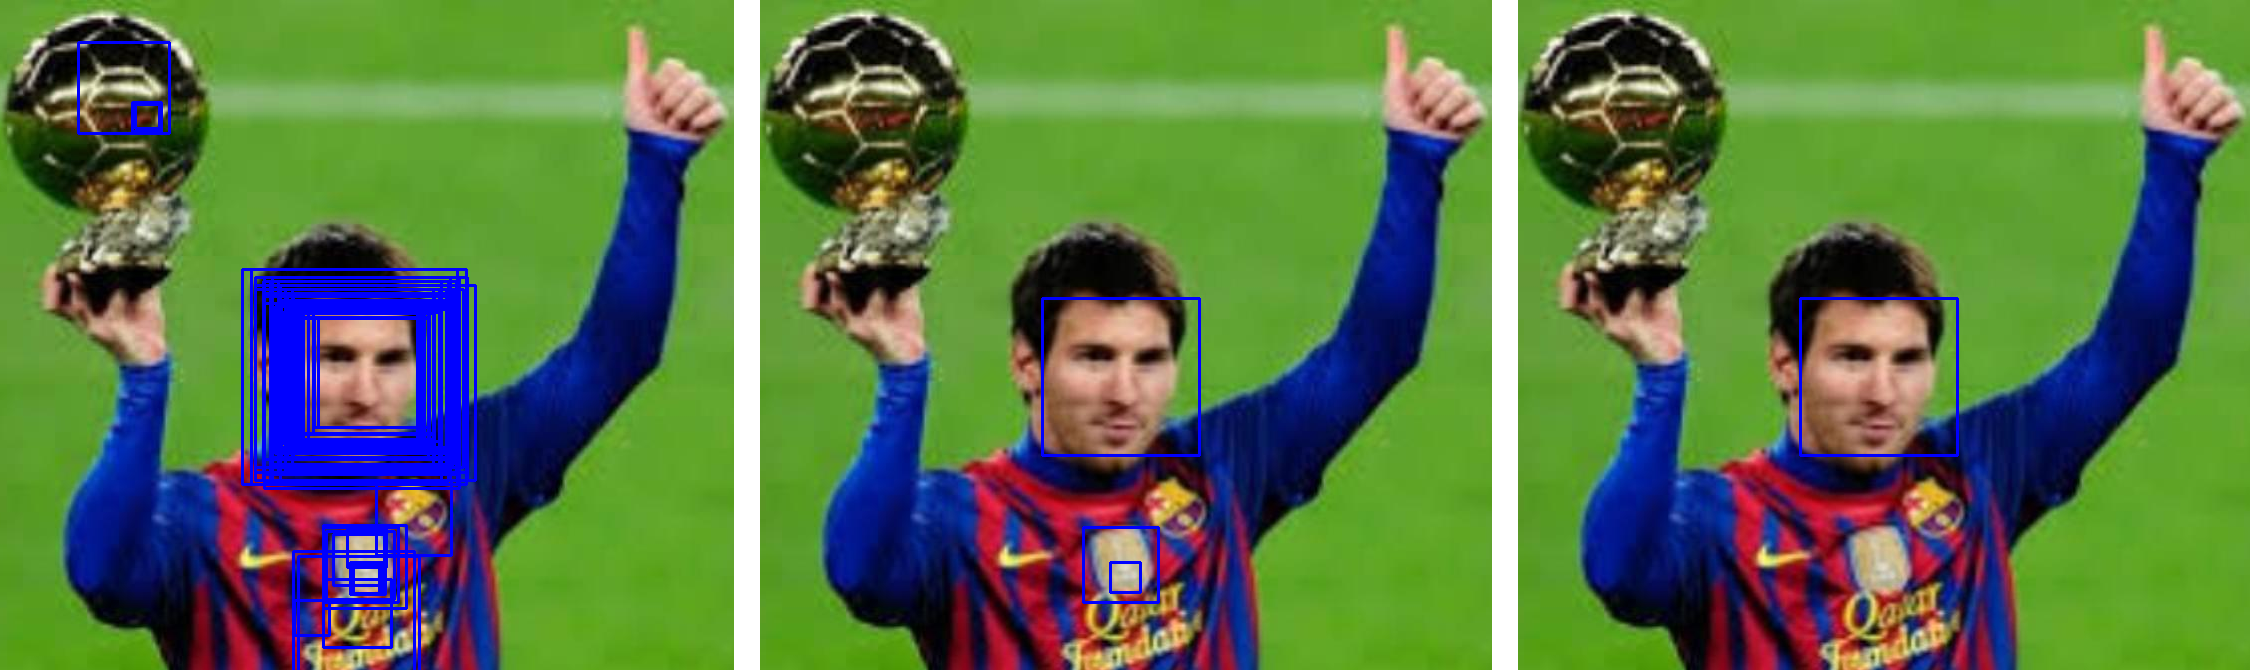
\includegraphics[scale=.2]{figs/min_neighbors_messi.png}
    \label{fig:min-neighbors-messi}
 \end{figure}

\section{KERAS PENDENTE}

Descrição MTCNN e Keras.

\section{Conjuntos de imagens para teste}

Para analisar a eficiência da implementação do algoritmo \textit{Viola-Jones} na biblioteca \textit{OpenCV}, assim como o seu modelo previamente treinado, foram selecionadas manualmente 500 imagens retiradas de dois conjuntos de imagens disponíveis na internet. 
 
\subsection{Conjuntos de imagens originais}

O primeiro conjunto de imagens, nomeado \textit{UTKFace}, disponível em \cite{utkface}, consiste em um conjunto de mais de 20 mil imagens, com uma única face em cada, de diversas pessoas entre 0 e 116 anos de idade, catalogadas de acordo com idade, raça e sexo. Alguns exemplos das imagens contidas no dataset podem ser vistos na figura \ref{fig:exemplos-utk}.

\begin{figure}[htb]
    \centering
    \caption{Exemplos de imagens do dataset \textit{UTKFace}.}
    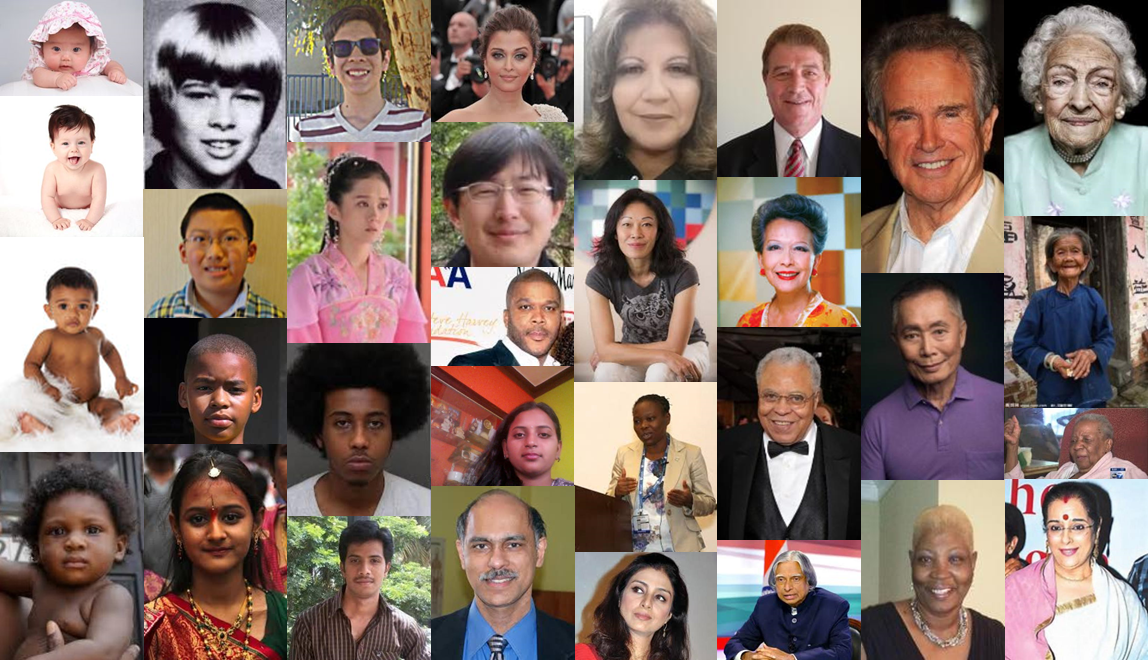
\includegraphics[scale=.3]{figs/exemplos-utk.png}
    \legend{Fonte: \textit{UTKFace dataset} \cite{utkface}}
    \label{fig:exemplos-utk}
 \end{figure}

 O segundo conjunto de imagens, nomeado \textit{Hotels-50k} \cite{hotels50k-article}, consistia originalmente em mais de 50 mil fotografias de diversos quartos de hotel vazios, este foi utilizado pois imagens com características semelhantes a estas são muitas vezes submetidas erroneamente em cadastros pessoais, ao invés de uma imagem da face a ser cadastrada.

\subsection{Conjunto de imagens selecionadas}

Para os testes, foi selecionado manualmente um conjunto com 400 positivas (possuíam uma face válida) e 100 imagens negativas (não possuíam uma face válida). Tal proporção representa a hipótese de que cerca de 20\% de imagens enviadas para cadastros na verdade não possuem uma face.

Por considerar que as imagens avaliadas pelo detector facial estudado neste trabalho serão utilizadas para cadastros pessoais e portanto é necessário que demonstrem que houve o consentimento de quem estava sendo fotografado e que seja possível identificar com clareza a pessoa da foto, as 400 imagens positivas (exemplos na figura \ref{fig:valid-faces}) foram selecionadas de forma que cumprissem os critérios abaixo.

\begin{itemize}
    \item A imagem deve conter uma única face frontal;
    \item Olhos, nariz e boca devem estar visíveis;
    \item A pessoa fotografada deve ter entre 18 e 60 anos;
    \item A pessoa fotografada deve estar olhando para a camera;
    \item A imagem deve ter boa definição e foco;
    \item A face deve estar centralizada e próxima da camera.
\end{itemize}

\begin{figure}[htbp]
    \centering
    \caption{Exemplos de imagens com face válida.}
    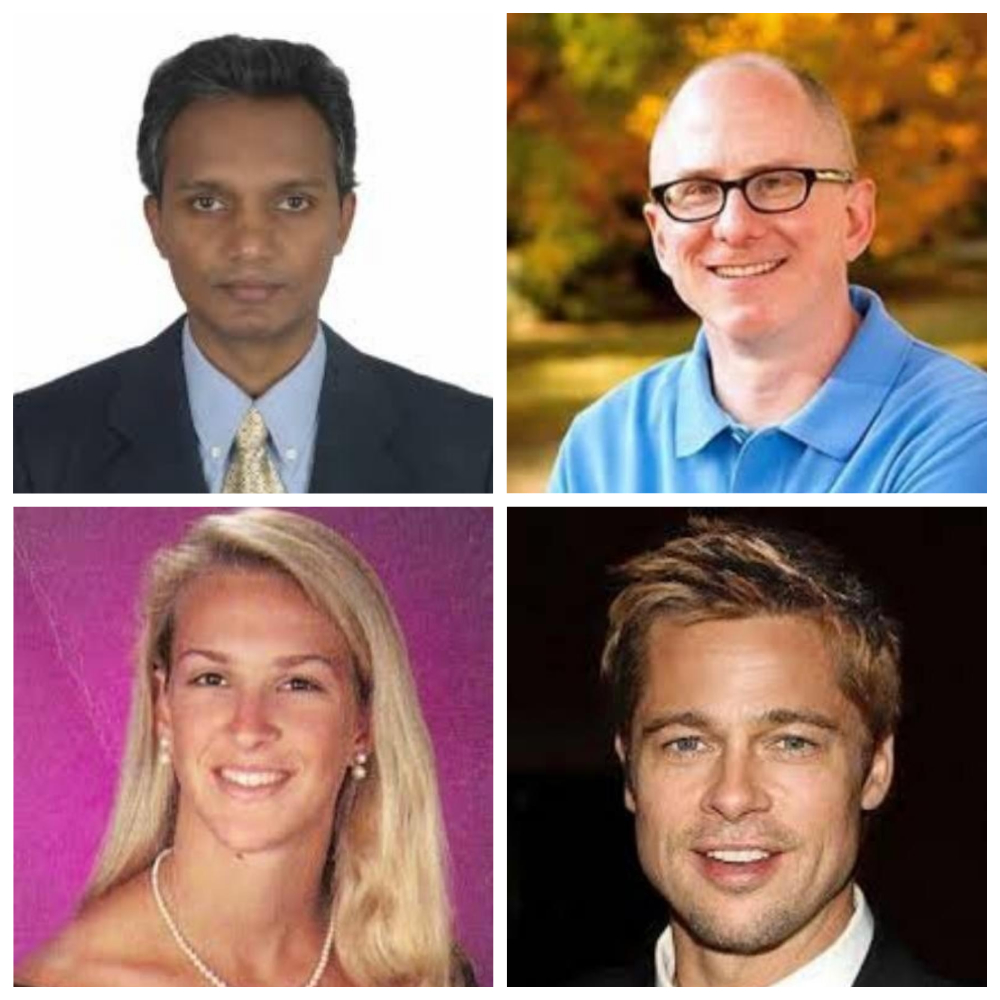
\includegraphics[scale=.25]{figs/valid_faces.jpg}
    \legend{Fonte: \textit{UTKFace dataset} \cite{utkface}}
    \label{fig:valid-faces}
 \end{figure}

É preciso considerar também que existem imagens que contém faces mas que não são válidas pois não cumprem os critérios definidos, portanto essas devem ser consideradas negativas. Para maior realidade nos testes feitos, o grupo de imagens negativas foi composto por 30 imagens que apresentavam faces inválidas (exemplos na figura \ref{fig:invalid-faces}) e outras 70 imagens selecionadas aleatoriamente do conjunto \textit{Hotels-50k} (exemplos na figura \ref{fig:hotel-examples}).

\begin{figure}[htbp]
    \centering
    \caption{Exemplos de imagens com face inválida.}
    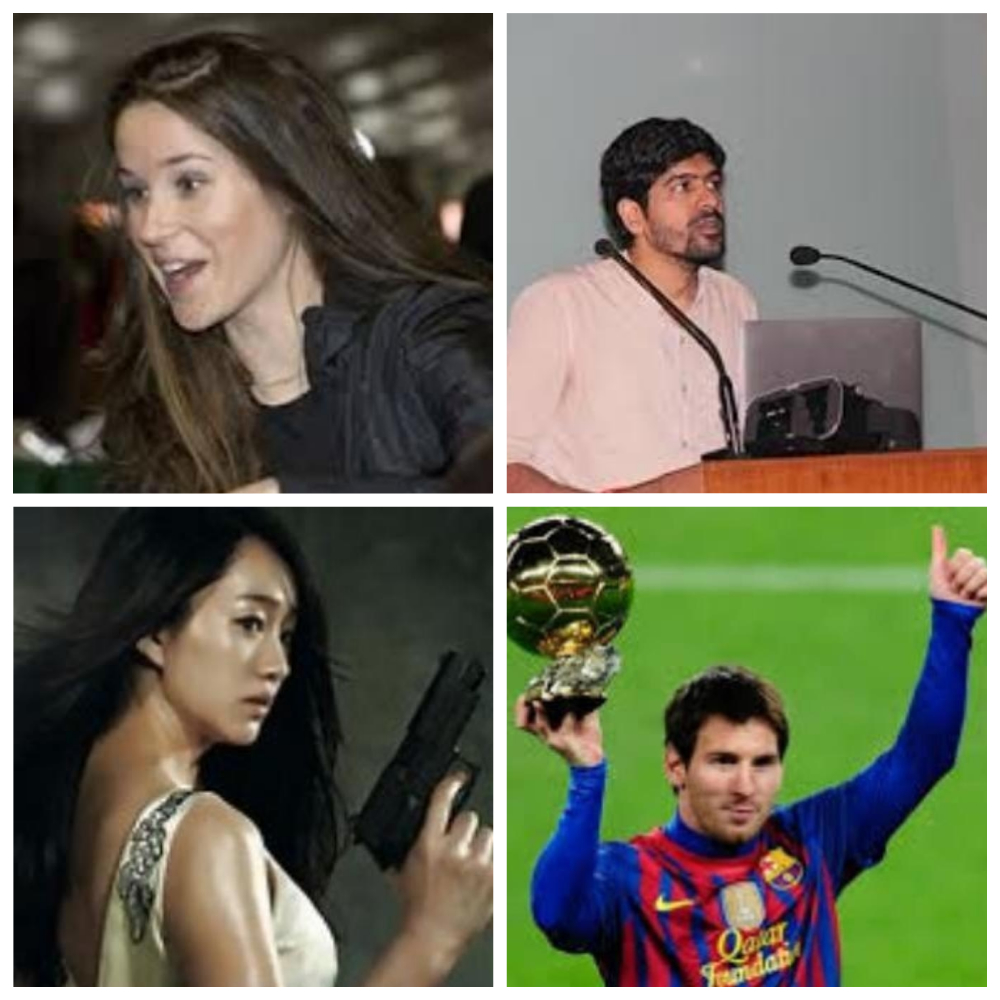
\includegraphics[scale=.25]{figs/invalid_faces.jpg}
    \legend{Fonte: \textit{UTKFace dataset} \cite{utkface}}
    \label{fig:invalid-faces}
 \end{figure}

 \begin{figure}[htbp]
     \centering
     \caption{Exemplos de imagens sem nenhuma face.}
     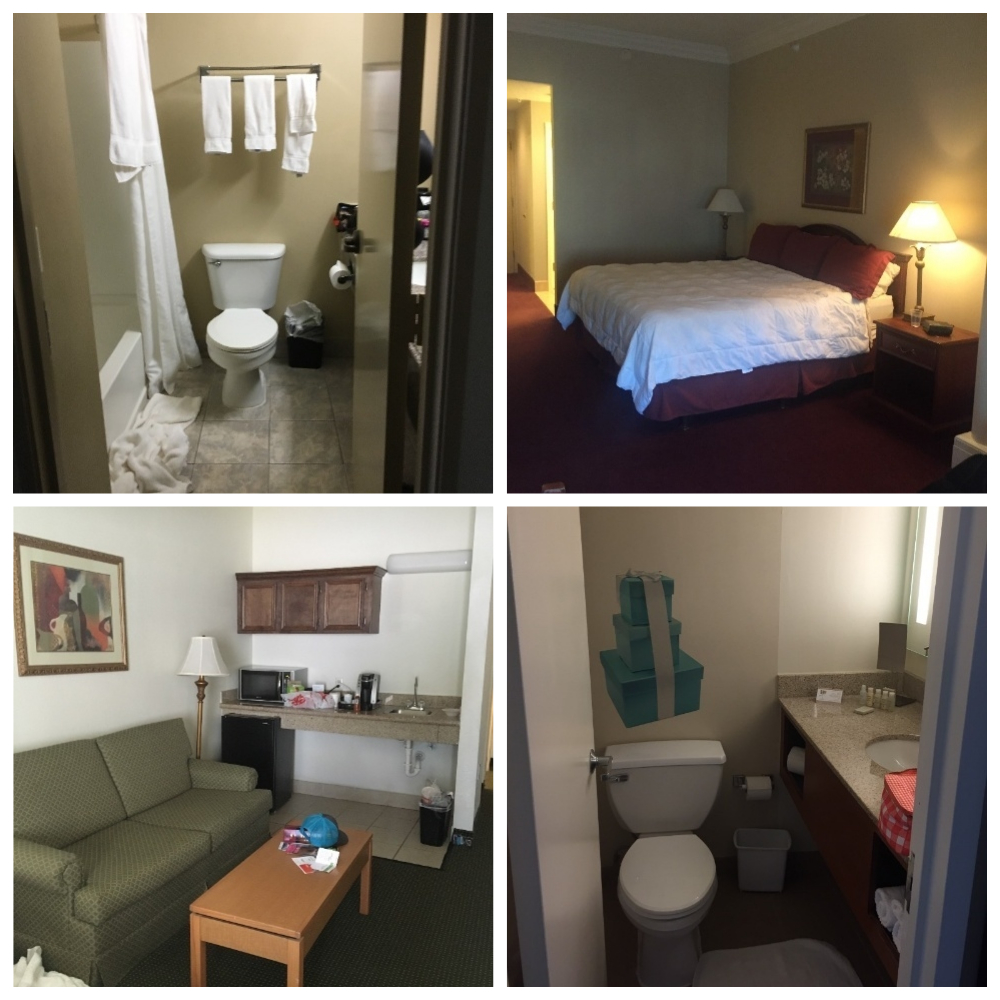
\includegraphics[scale=.25]{figs/hotels.jpg}
     \legend{Fonte: \textit{Hotels-50k dataset} \cite{hotels50k-article}}
     \label{fig:hotel-examples}
  \end{figure}

%-
\section{Metodologia de Análise}
%-

Para melhor analisar os resultados dos testes, foi necessário especificar com clareza como poderiam ser agrupadas as imagens, dada a sua origem e o resultado observado no teste, para isso foram utilizadas as definições da Tabela \ref{tab:grupos-images}. 

\begin{table}[htbp]
    \caption{Grupos observados}
    \label{tab:grupos-images}
    \centering
    \begin{tabular}{ccc}\hline\hline
        \textbf{Grupo} & \textbf{Descrição} & \textbf{Quantidade} \\\hline
        \textit{A} & Imagens que contêm uma face válida & 400 \\
        $\overline{A}$ & Imagens que não contêm uma face válida & 100 \\
        \textit{B} & Imagens onde o algoritmo identificou uma ou mais faces & Variável \\
        $\overline{B}$ & Imagens onde o algoritmo não identificou nenhuma face & Variável \\
    \hline\hline
    \end{tabular}
\end{table}

Definidos os grupos, pode-se utilizar a matriz de confusão da Tabela \ref{tab:matriz_de_confusao} para facilitar a análise da relação entre os grupos definidos anteriormente. Na Tabela \ref{tab:matriz_de_confusao} são observados os grupos \textit{a - verdadeiro positivo} (TP, \textit{true positive}) onde o algoritmo identifica corretamente uma face em cada uma das imagens que realmente contêm uma face, \textit{b - falso negativo} (FN, \textit{false negative}) onde o algoritmo erroneamente não reconheceu nenhuma face, apesar das imagens conterem uma face cada, \textit{c - falso positivo} (FP, \textit{false positive}) onde o algoritmo erroneamente identificou ao menos uma face, mesmo as imagens não contendo nenhuma e \textit{d - verdadeiro negativo} (TN, \textit{true negative}) onde o algoritmo identificou corretamente que não existia nenhuma face nas imagens. É importante destacar que os quatro grupos destacados na matriz de confusão são mutuamente excludentes \cite{Dougherty:2012:PRC:2553126}.

\begin{table}[htbp]
    \caption{Matriz de confusão}
    \label{tab:matriz_de_confusao}
    \centering
    \begin{tabular}{ccc}\hline\hline
        & \textit{B} & $\overline{B}$ \\
    \textit{A} & \textit{a} (verdadeiro positivo) & \textit{b} (falso negativo) \\
    $\overline{A}$ & \textit{c} (falso positivo) & \textit{d} (verdadeiro negativo) \\
    \hline\hline
    \end{tabular}
\end{table}

Para melhor entender os agrupamentos da matriz de confusão, pode-se observar na Figura \ref{fig:norm_dist} as distribuições que representam a quantidade de imagens dos grupos \textit{A} e $\overline{A}$ dada a sua probabilidade de conter uma face. 

\begin{figure}[htbp]
    \centering
    \caption{Exemplo teórico de uma distribuição normal dos grupos de uma matriz de confusão.}
    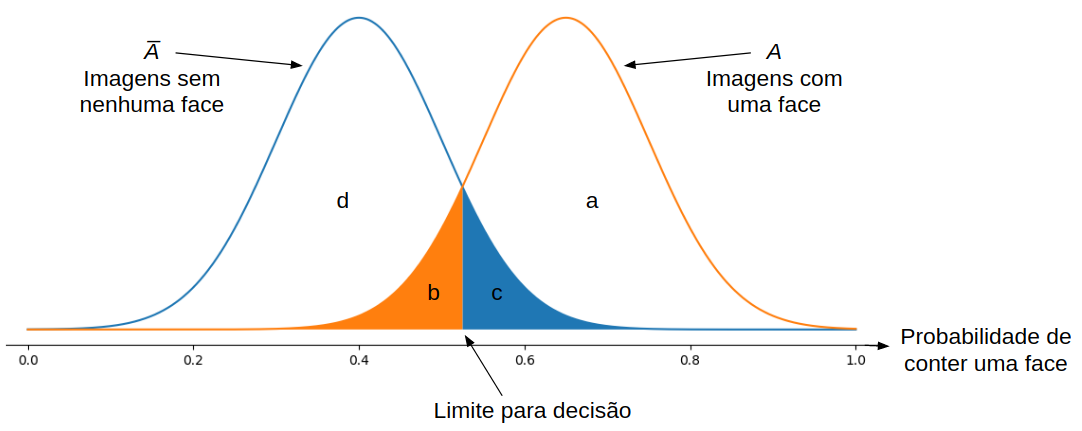
\includegraphics[scale=.4]{figs/norm_dist.png}
    \label{fig:norm_dist}
 \end{figure}

 Nas distribuições são destacados os grupos \textit{b} (falso negativo) e \textit{c} (falso positivo) e fica evidente que, devido a sobreposição das distribuições \textit{A} e $\overline{A}$, é necessário definir uma limite para decisão, que pode ser ajustado conforme a necessidade, mas que independente do seu ajuste, sempre existirá um grupo categorizado de forma incorreta.

 A matriz de confusão também pode ser escrita em termos probabilísticos (Tabela \ref{tab:matriz_de_confusao_probab}), incluindo as probabilidades marginais ou pode ser visualizada no diagrama de Venn correspondente (Figura \ref{fig:venn_diagram}).

\begin{table}[htbp]
    \caption{Matriz de confusão com probabilidades marginais}
    \label{tab:matriz_de_confusao_probab}
    \centering
    \begin{tabular}{cccc}\hline\hline
        & \textit{B} & $\overline{B}$ & Soma\\
    \textit{A} & $P(A \cap B)$ & $P(A \cap \overline{B})$ & $P(A)$ \\
    $\overline{A}$ & $P(\overline{A} \cap B)$ & $P(\overline{A} \cap \overline{B})$ & $P(\overline{A})$ \\
    Soma & $P(B)$ & $P(\overline{B})$ & 1 \\
    \hline\hline
    \end{tabular}
\end{table}

\begin{figure}[htbp]
    \centering
    \caption{Diagrama de Venn para as imagens analisadas.}
    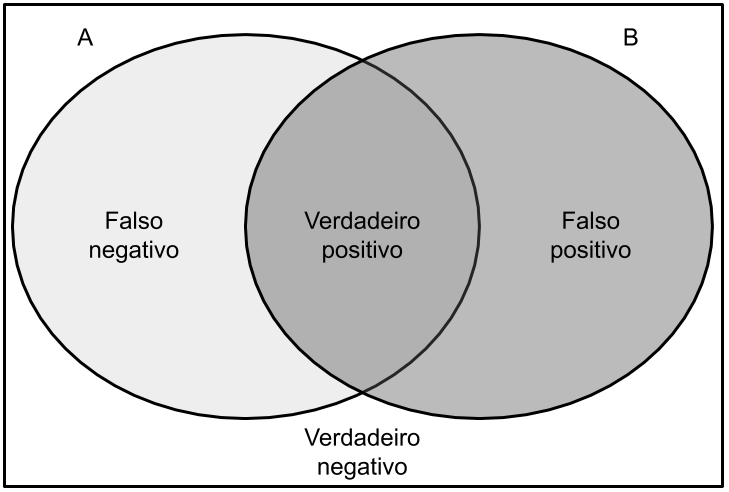
\includegraphics[scale=.4]{figs/venn-diagram.png}
    \label{fig:venn_diagram}
\end{figure}

Podem também ser calculadas as medidas tradicionais de sensitividade (a probabilidade condicional do algoritmo identificar ao menos uma face dado que a imagem contém uma face) e especificidade (a probabilidade condicional do algoritmo não identificar nenhuma face em uma imagem que realmente não contém nenhuma face) conforme as equações \ref{eq:sensitividade} e \ref{eq:especificidade}.

\begin{align} \label{eq:sensitividade}
    \text{sensitividade, } P(B|A) = P(A \cap B) / (P(A \cap B) + P(A \cap \overline{B})) = a/(a + b) \\
    \label{eq:especificidade}
    \text{especificidade, } P(\overline{B} | \overline{A}) = P(\overline{A} \cap \overline{B}) / (P(\overline{A} \cap \overline{B}) + P(\overline{A} \cap B)) = d/(d + c)
\end{align}

Por fim, a partir da sensitividade e especificidade é possível exibir o resultado do classificador no espaço ROC (\textit{Receiver Operating Characteristic}, traduzido literalmente como Característica operacional do receptor), que consiste em um plano onde o eixo horizontal mede a taxa de falsos positivos (1 - especificidade) e o eixo vertical mede a taxa de verdadeiros positivos (sensitividade), isso permite comparar facilmente diferentes classificadores, pois quanto mais próximo do canto esquerdo superior, melhor a classificação.

\begin{figure}[htbp]
    \centering
    \caption{Espaço ROC.}
    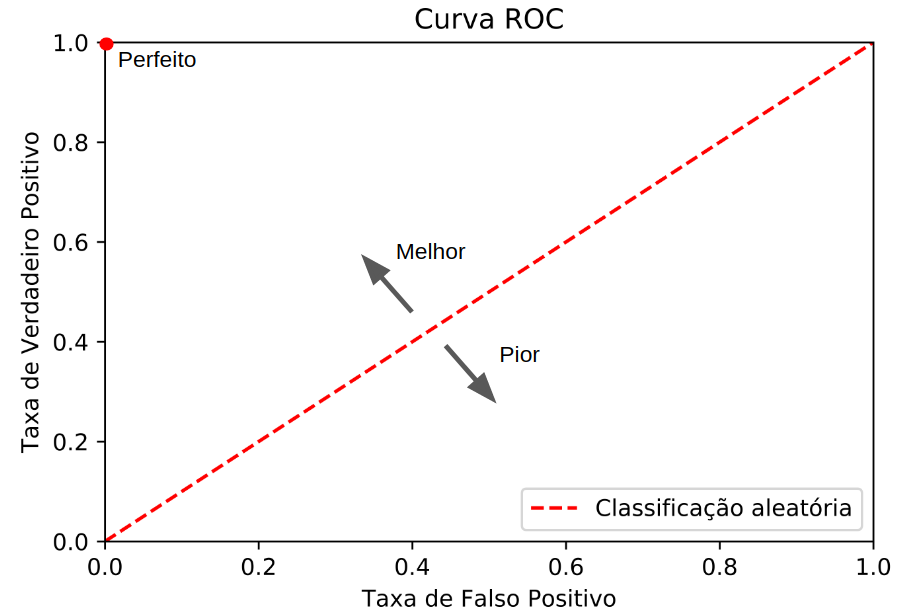
\includegraphics[scale=.4]{figs/curva_roc.png}
    \label{fig:roc_space}
\end{figure}

\section{Análise de Custo}

Para entender o valor da utilização de um modelo de reconhecimento facial para filtragem de imagens inválidas, pode-se utilizar o exemplo de uma empresa de cartões de crédito que precisa analisar fotos de clientes antes de fornecer um cartão para os mesmos. Considerando como R o valor presente líquido \cite{npv-article}, ou seja, a receita total que este cliente traz para empresa, e H como o custo de trabalho humano para a análise de uma imagem, podemos calcular a receita da empresa antes e depois da aplicação de um modelo de detecção facial.

Antes da aplicação do modelo, todas as fotos enviadas deveriam ser analisadas por um humano, gerando o custo de análise manual H, e apenas as fotos que continham uma face trariam a receita R para empresa, relacionando isso aos valores encontrados na matriz de confusão do modelo, pode-se obter a equação \ref{eq:g_0}. Nesta equação tem-se o $Evento\:A = (TP + FN)$, que representa os casos onde uma foto que realmente contém uma face, multiplicado pela receita de cada cliente R, subtraídos do custo de análise H multiplicado pela quantidade total de fotos recebidas, que equivale a soma de todas as taxas da matriz de confusão.

\begin{align} \label{eq:g_0}
    g_0 = (TP+FN) \times R - (TP+FP+FN+TN) \times H
\end{align}

Após a aplicação do modelo, apenas as fotos que foram classificadas pelo modelo como faces serão analisadas por humanos, gerando custo de análise manual H e apenas as fotos classificadas pelo modelo como face e que realmente contenham uma face se tornarão clientes reais, trazendo receita R para a empresa, com isso, pode-se obter a equação \ref{eq:g_1}.
\begin{align} \label{eq:g_1}
    g_1 = TP \times R - (TP+FP) \times H
\end{align}

Para avaliar a receita que o modelo traz para a empresa, pode-se calcular a diferença entre a receita antes e depois do modelo, obtendo a equação \ref{eq:profit}.
\begin{align} \label{eq:profit}
    g_1 - g_0 = (FN + TN) \times H - FN \times R
\end{align}

Considerando que para o modelo trazer valor para a empresa, é necessário que a receita após sua aplicação seja maior que a receita antes da sua aplicação, obtendo a equação \ref{eq:profit2}.
\begin{align} \label{eq:profit2}
    g_1 - g_0 > 0 \\
    (FN + TN) \times H - FN \times R > 0
\end{align}

A equação obtida ainda pode ser reescrita em função da \textit{taxa de verdadeiros positivos} (TPR, \textit{true positive rate}) e da taxa de falsos positivos (FPR, \textit{false positive rate}) de forma que seja possível traça-la sobre o espaço ROC e visualizar de forma simples quais classificadores satisfazem o critério necessário para obtenção de receita. Para isso são consideradas a quantidade de imagens positivas ($ P = 0.8 $) e negativas ($ N = 0.2 $) definidas anteriormente e as relações \ref{eq:FN_TPR} e \ref{eq:TN_FPR}, obtendo por fim a equação \ref{eq:profit_roc} que pode ser exibida no espaço ROC em \ref{fig:profit_roc}.

\begin{align} 
    \label{eq:FN_TPR}
    FN &= P \times (1-TPR) \\
    \label{eq:TN_FPR}
    TN &= N \times (1-FPR) \\
    \label{eq:profit_roc}
    TPR &= 1 + \left( \frac{N}{P \times \left( \frac{R}{H}-1 \right) } \times (FPR - 1) \right)
\end{align}

\begin{figure}[htbp]
    \centering
    \caption{Limiar lucrativo exibido no espaço ROC.}
    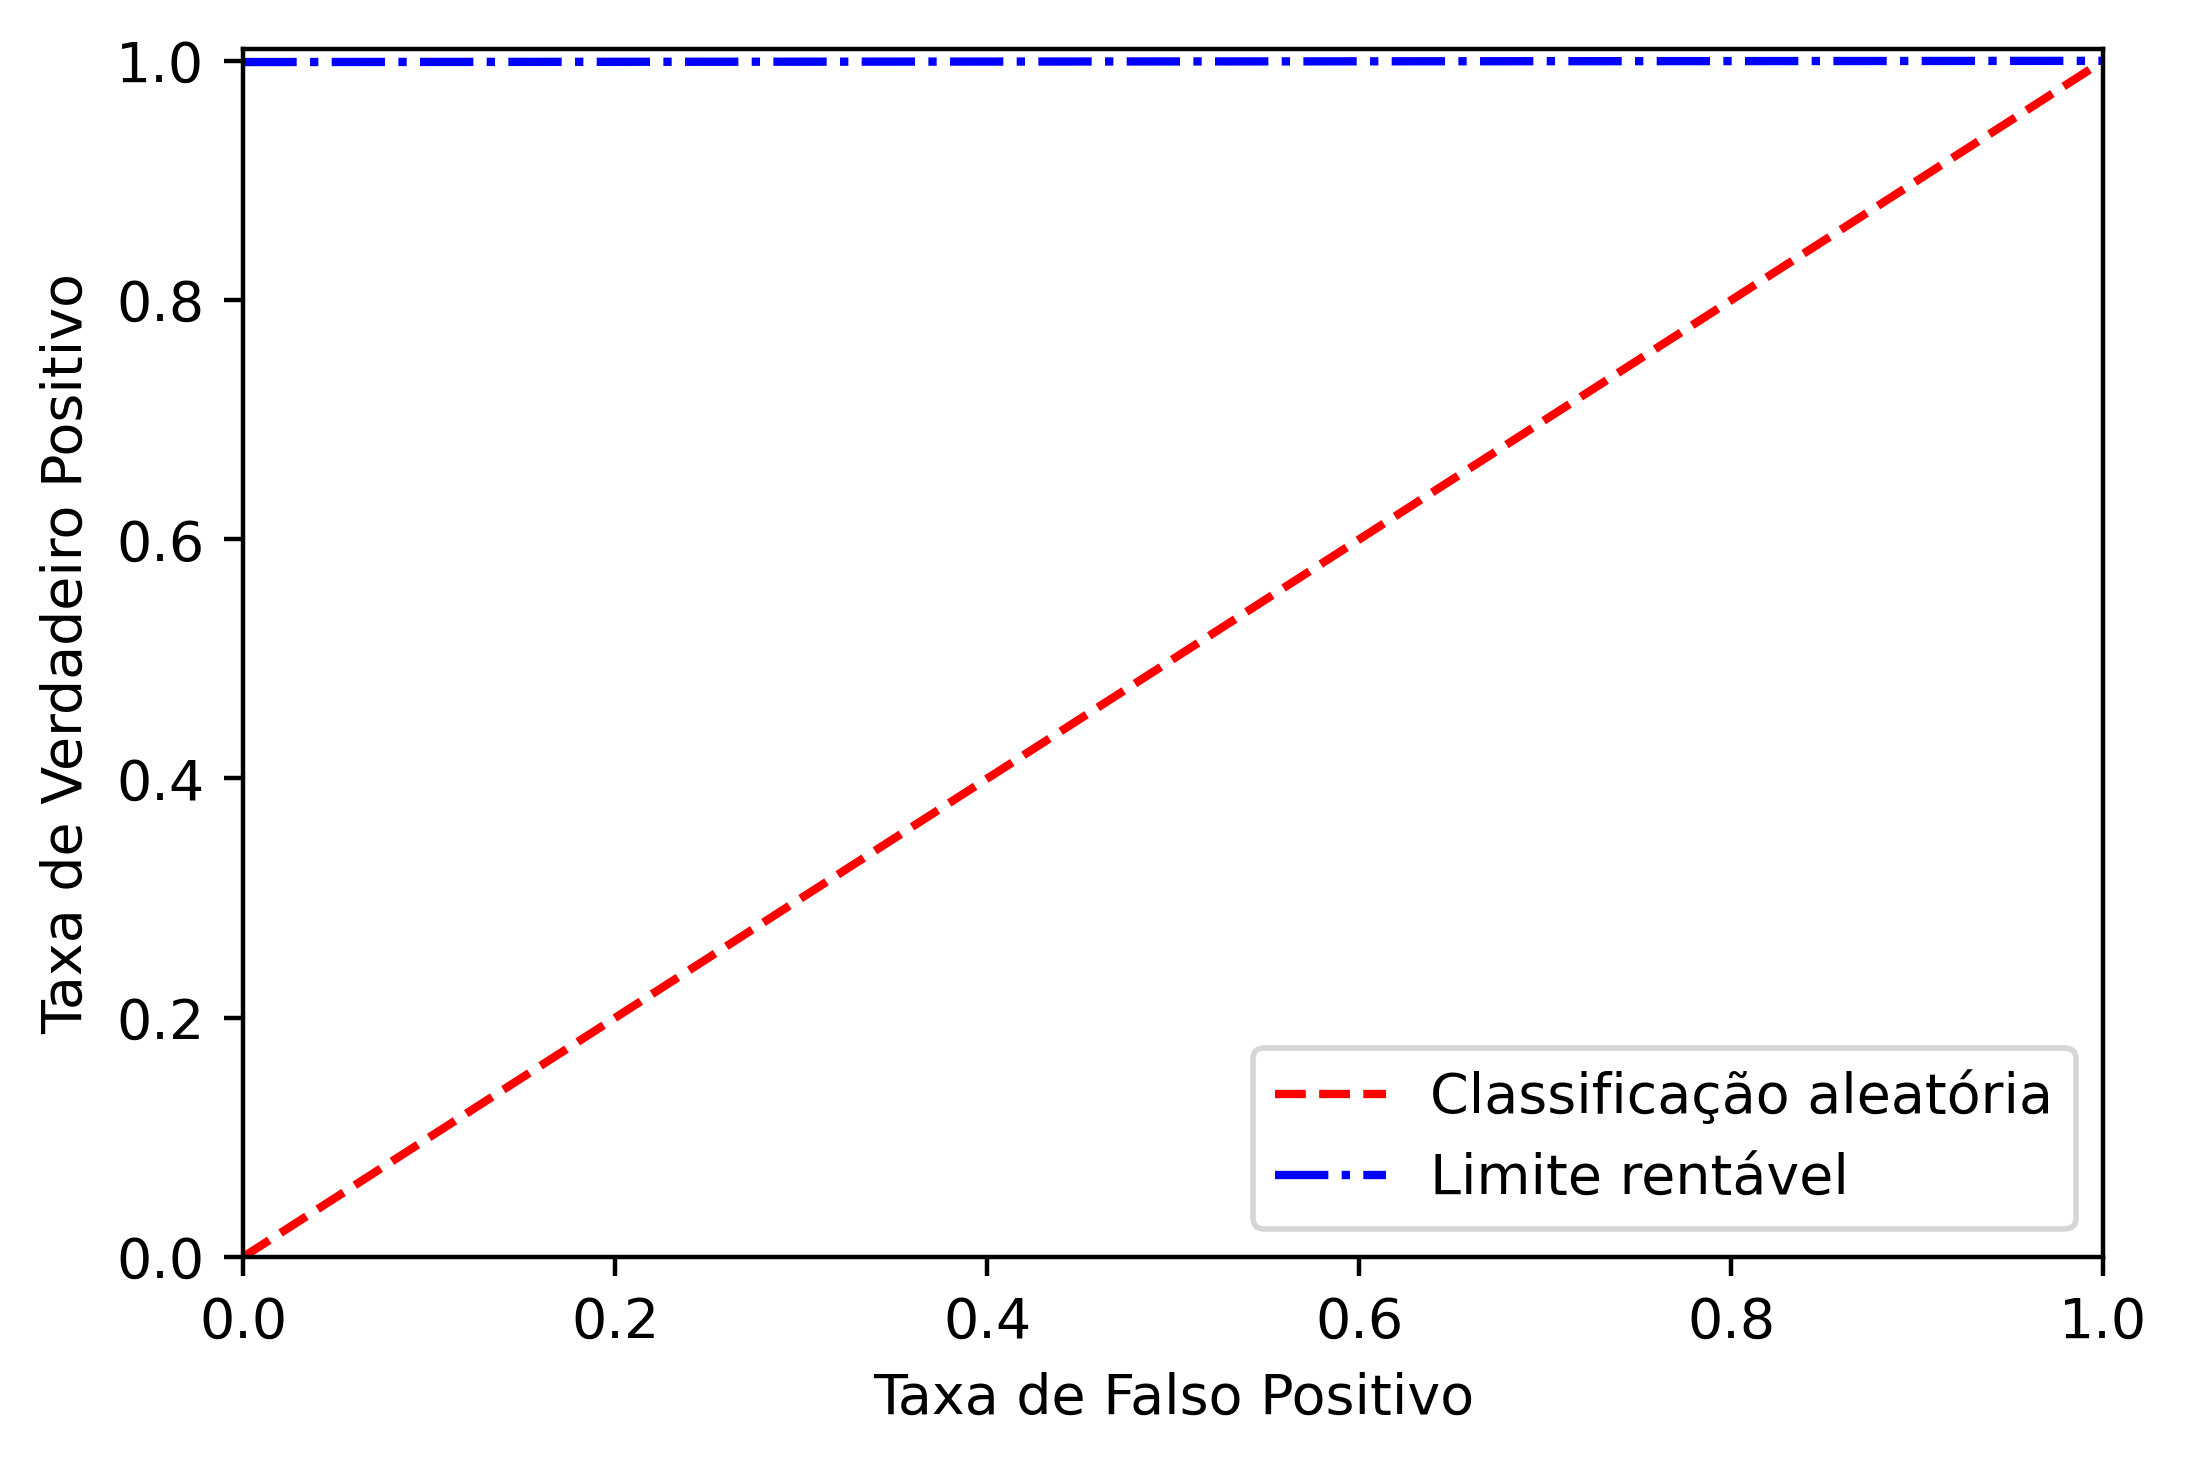
\includegraphics[scale=1]{figs/curva_roc_lucro.png}
    \label{fig:profit_roc}
\end{figure}

Assim, é possível avaliar em função da matriz de confusão do modelo, do custo de análise manual de um documento, do valor presente líquido de um cliente e da proporção média de imagens positivas e negativas, se a aplicação deste modelo é viável ou não.
